% Created 2024-11-18 Mon 13:59
% Intended LaTeX compiler: pdflatex
\documentclass[11pt]{article}
\usepackage[utf8]{inputenc}
\usepackage[T1]{fontenc}
\usepackage{graphicx}
\usepackage{longtable}
\usepackage{wrapfig}
\usepackage{rotating}
\usepackage[normalem]{ulem}
\usepackage{amsmath}
\usepackage{amssymb}
\usepackage{capt-of}
\usepackage{hyperref}
\usepackage[polish]{babel}
\usepackage[T1]{fontenc}
\usepackage[utf8]{inputenc}
\selectlanguage{polish}
\usepackage{caption}
\usepackage{booktabs}
\captionsetup{labelfont=bf}
\usepackage{float}
\usepackage[a4paper, total={7in, 9in}]{geometry}
\author{Piotr Karamon}
\date{18.11.2024r.}
\title{Laboratorium 6 - Problem czytelników i pisarzy}
\hypersetup{
 pdfauthor={Piotr Karamon},
 pdftitle={Laboratorium 6 - Problem czytelników i pisarzy},
 pdfkeywords={},
 pdfsubject={},
 pdfcreator={Emacs 29.2 (Org mode 9.7.11)}, 
 pdflang={Polish}}

% Setup for code blocks [1/2]

\usepackage{fvextra}

\fvset{%
  commandchars=\\\{\},
  highlightcolor=white!95!black!80!blue,
  breaklines=true,
  breaksymbol=\color{white!60!black}\tiny\ensuremath{\hookrightarrow}}

% Make line numbers smaller and grey.
\renewcommand\theFancyVerbLine{\footnotesize\color{black!40!white}\arabic{FancyVerbLine}}

\usepackage{xcolor}

% In case engrave-faces-latex-gen-preamble has not been run.
\providecolor{EfD}{HTML}{f7f7f7}
\providecolor{EFD}{HTML}{28292e}

% Define a Code environment to prettily wrap the fontified code.
\usepackage[breakable,xparse]{tcolorbox}
\DeclareTColorBox[]{Code}{o}%
{colback=EfD!98!EFD, colframe=EfD!95!EFD,
  fontupper=\footnotesize\setlength{\fboxsep}{0pt},
  colupper=EFD,
  IfNoValueTF={#1}%
  {boxsep=2pt, arc=2.5pt, outer arc=2.5pt,
    boxrule=0.5pt, left=2pt}%
  {boxsep=2.5pt, arc=0pt, outer arc=0pt,
    boxrule=0pt, leftrule=1.5pt, left=0.5pt},
  right=2pt, top=1pt, bottom=0.5pt,
  breakable}

% Support listings with captions
\usepackage{float}
\floatstyle{plain}
\newfloat{listing}{htbp}{lst}
\newcommand{\listingsname}{Listing}
\floatname{listing}{\listingsname}
\newcommand{\listoflistingsname}{List of Listings}
\providecommand{\listoflistings}{\listof{listing}{\listoflistingsname}}


% Setup for code blocks [2/2]: syntax highlighting colors

\newcommand\efstrut{\vrule height 2.1ex depth 0.8ex width 0pt}
\definecolor{EFD}{HTML}{000000}
\definecolor{EfD}{HTML}{ffffff}
\newcommand{\EFD}[1]{\textcolor{EFD}{#1}} % default
\newcommand{\EFvp}[1]{#1} % variable-pitch
\definecolor{EFh}{HTML}{595959}
\newcommand{\EFh}[1]{\textcolor{EFh}{#1}} % shadow
\definecolor{EFsc}{HTML}{005f5f}
\newcommand{\EFsc}[1]{\textcolor{EFsc}{\textbf{#1}}} % success
\definecolor{EFw}{HTML}{884900}
\newcommand{\EFw}[1]{\textcolor{EFw}{\textbf{#1}}} % warning
\definecolor{EFe}{HTML}{a60000}
\newcommand{\EFe}[1]{\textcolor{EFe}{\textbf{#1}}} % error
\definecolor{EFl}{HTML}{3548cf}
\newcommand{\EFl}[1]{\textcolor{EFl}{#1}} % link
\definecolor{EFlv}{HTML}{721045}
\newcommand{\EFlv}[1]{\textcolor{EFlv}{#1}} % link-visited
\definecolor{Efhi}{HTML}{b2e4dc}
\newcommand{\EFhi}[1]{\colorbox{Efhi}{\efstrut{}#1}} % highlight
\definecolor{EFc}{HTML}{595959}
\newcommand{\EFc}[1]{\textcolor{EFc}{\textit{#1}}} % font-lock-comment-face
\definecolor{EFcd}{HTML}{595959}
\newcommand{\EFcd}[1]{\textcolor{EFcd}{\textit{#1}}} % font-lock-comment-delimiter-face
\definecolor{EFs}{HTML}{3548cf}
\newcommand{\EFs}[1]{\textcolor{EFs}{#1}} % font-lock-string-face
\definecolor{EFd}{HTML}{2a5045}
\newcommand{\EFd}[1]{\textcolor{EFd}{\textit{#1}}} % font-lock-doc-face
\definecolor{EFm}{HTML}{7c318f}
\newcommand{\EFm}[1]{\textcolor{EFm}{\textit{#1}}} % font-lock-doc-markup-face
\definecolor{EFk}{HTML}{531ab6}
\newcommand{\EFk}[1]{\textcolor{EFk}{#1}} % font-lock-keyword-face
\definecolor{EFb}{HTML}{8f0075}
\newcommand{\EFb}[1]{\textcolor{EFb}{#1}} % font-lock-builtin-face
\definecolor{EFf}{HTML}{721045}
\newcommand{\EFf}[1]{\textcolor{EFf}{#1}} % font-lock-function-name-face
\definecolor{EFv}{HTML}{005e8b}
\newcommand{\EFv}[1]{\textcolor{EFv}{#1}} % font-lock-variable-name-face
\definecolor{EFt}{HTML}{005f5f}
\newcommand{\EFt}[1]{\textcolor{EFt}{#1}} % font-lock-type-face
\definecolor{EFo}{HTML}{0000b0}
\newcommand{\EFo}[1]{\textcolor{EFo}{#1}} % font-lock-constant-face
\definecolor{EFwr}{HTML}{884900}
\newcommand{\EFwr}[1]{\textcolor{EFwr}{#1}} % font-lock-warning-face
\definecolor{EFnc}{HTML}{a60000}
\newcommand{\EFnc}[1]{\textcolor{EFnc}{\textbf{#1}}} % font-lock-negation-char-face
\definecolor{EFpp}{HTML}{a0132f}
\newcommand{\EFpp}[1]{\textcolor{EFpp}{#1}} % font-lock-preprocessor-face
\definecolor{EFrc}{HTML}{00663f}
\newcommand{\EFrc}[1]{\textcolor{EFrc}{#1}} % font-lock-regexp-grouping-construct
\definecolor{EFrb}{HTML}{721045}
\newcommand{\EFrb}[1]{\textcolor{EFrb}{#1}} % font-lock-regexp-grouping-backslash
\definecolor{Efob}{HTML}{f2f2f2}
\newcommand{\EFob}[1]{\colorbox{Efob}{\efstrut{}#1}} % org-block
\definecolor{EFobb}{HTML}{595959}
\definecolor{Efobb}{HTML}{f2f2f2}
\newcommand{\EFobb}[1]{\colorbox{Efobb}{\efstrut{}\textcolor{EFobb}{#1}}} % org-block-begin-line
\definecolor{EFobe}{HTML}{595959}
\definecolor{Efobe}{HTML}{f2f2f2}
\newcommand{\EFobe}[1]{\colorbox{Efobe}{\efstrut{}\textcolor{EFobe}{#1}}} % org-block-end-line
\newcommand{\EFOa}[1]{\textbf{#1}} % outline-1
\definecolor{EFOb}{HTML}{624416}
\newcommand{\EFOb}[1]{\textcolor{EFOb}{\textbf{#1}}} % outline-2
\definecolor{EFOc}{HTML}{193668}
\newcommand{\EFOc}[1]{\textcolor{EFOc}{\textbf{#1}}} % outline-3
\definecolor{EFOd}{HTML}{721045}
\newcommand{\EFOd}[1]{\textcolor{EFOd}{\textbf{#1}}} % outline-4
\definecolor{EFOe}{HTML}{2a5045}
\newcommand{\EFOe}[1]{\textcolor{EFOe}{\textbf{#1}}} % outline-5
\definecolor{EFOf}{HTML}{7f0000}
\newcommand{\EFOf}[1]{\textcolor{EFOf}{\textbf{#1}}} % outline-6
\definecolor{EFOg}{HTML}{3f578f}
\newcommand{\EFOg}[1]{\textcolor{EFOg}{\textbf{#1}}} % outline-7
\definecolor{EFOh}{HTML}{595959}
\newcommand{\EFOh}[1]{\textcolor{EFOh}{\textbf{#1}}} % outline-8
\definecolor{EFhn}{HTML}{0000b0}
\newcommand{\EFhn}[1]{\textcolor{EFhn}{#1}} % highlight-numbers-number
\newcommand{\EFhq}[1]{#1} % highlight-quoted-quote
\newcommand{\EFhs}[1]{#1} % highlight-quoted-symbol
\newcommand{\EFrda}[1]{#1} % rainbow-delimiters-depth-1-face
\definecolor{EFrdb}{HTML}{dd22dd}
\newcommand{\EFrdb}[1]{\textcolor{EFrdb}{#1}} % rainbow-delimiters-depth-2-face
\definecolor{EFrdc}{HTML}{008899}
\newcommand{\EFrdc}[1]{\textcolor{EFrdc}{#1}} % rainbow-delimiters-depth-3-face
\definecolor{EFrdd}{HTML}{972500}
\newcommand{\EFrdd}[1]{\textcolor{EFrdd}{#1}} % rainbow-delimiters-depth-4-face
\definecolor{EFrde}{HTML}{808000}
\newcommand{\EFrde}[1]{\textcolor{EFrde}{#1}} % rainbow-delimiters-depth-5-face
\definecolor{EFrdf}{HTML}{531ab6}
\newcommand{\EFrdf}[1]{\textcolor{EFrdf}{#1}} % rainbow-delimiters-depth-6-face
\definecolor{EFrdg}{HTML}{008900}
\newcommand{\EFrdg}[1]{\textcolor{EFrdg}{#1}} % rainbow-delimiters-depth-7-face
\definecolor{EFrdh}{HTML}{3548cf}
\newcommand{\EFrdh}[1]{\textcolor{EFrdh}{#1}} % rainbow-delimiters-depth-8-face
\definecolor{EFrdi}{HTML}{8f0075}
\newcommand{\EFrdi}[1]{\textcolor{EFrdi}{#1}} % rainbow-delimiters-depth-9-face
\definecolor{EFany}{HTML}{6f5500}
\definecolor{Efany}{HTML}{6f5500}
\newcommand{\EFany}[1]{\colorbox{Efany}{\efstrut{}\textcolor{EFany}{#1}}} % ansi-color-yellow
\definecolor{EFanr}{HTML}{a60000}
\definecolor{Efanr}{HTML}{a60000}
\newcommand{\EFanr}[1]{\colorbox{Efanr}{\efstrut{}\textcolor{EFanr}{#1}}} % ansi-color-red
\definecolor{EFanb}{HTML}{000000}
\definecolor{Efanb}{HTML}{000000}
\newcommand{\EFanb}[1]{\colorbox{Efanb}{\efstrut{}\textcolor{EFanb}{#1}}} % ansi-color-black
\definecolor{EFang}{HTML}{006800}
\definecolor{Efang}{HTML}{006800}
\newcommand{\EFang}[1]{\colorbox{Efang}{\efstrut{}\textcolor{EFang}{#1}}} % ansi-color-green
\definecolor{EFanB}{HTML}{0031a9}
\definecolor{EfanB}{HTML}{0031a9}
\newcommand{\EFanB}[1]{\colorbox{EfanB}{\efstrut{}\textcolor{EFanB}{#1}}} % ansi-color-blue
\definecolor{EFanc}{HTML}{005e8b}
\definecolor{Efanc}{HTML}{005e8b}
\newcommand{\EFanc}[1]{\colorbox{Efanc}{\efstrut{}\textcolor{EFanc}{#1}}} % ansi-color-cyan
\definecolor{EFanw}{HTML}{a6a6a6}
\definecolor{Efanw}{HTML}{a6a6a6}
\newcommand{\EFanw}[1]{\colorbox{Efanw}{\efstrut{}\textcolor{EFanw}{#1}}} % ansi-color-white
\definecolor{EFanm}{HTML}{721045}
\definecolor{Efanm}{HTML}{721045}
\newcommand{\EFanm}[1]{\colorbox{Efanm}{\efstrut{}\textcolor{EFanm}{#1}}} % ansi-color-magenta
\definecolor{EFANy}{HTML}{884900}
\definecolor{EfANy}{HTML}{884900}
\newcommand{\EFANy}[1]{\colorbox{EfANy}{\efstrut{}\textcolor{EFANy}{#1}}} % ansi-color-bright-yellow
\definecolor{EFANr}{HTML}{972500}
\definecolor{EfANr}{HTML}{972500}
\newcommand{\EFANr}[1]{\colorbox{EfANr}{\efstrut{}\textcolor{EFANr}{#1}}} % ansi-color-bright-red
\definecolor{EFANb}{HTML}{595959}
\definecolor{EfANb}{HTML}{595959}
\newcommand{\EFANb}[1]{\colorbox{EfANb}{\efstrut{}\textcolor{EFANb}{#1}}} % ansi-color-bright-black
\definecolor{EFANg}{HTML}{00663f}
\definecolor{EfANg}{HTML}{00663f}
\newcommand{\EFANg}[1]{\colorbox{EfANg}{\efstrut{}\textcolor{EFANg}{#1}}} % ansi-color-bright-green
\definecolor{EFANB}{HTML}{3548cf}
\definecolor{EfANB}{HTML}{3548cf}
\newcommand{\EFANB}[1]{\colorbox{EfANB}{\efstrut{}\textcolor{EFANB}{#1}}} % ansi-color-bright-blue
\definecolor{EFANc}{HTML}{005f5f}
\definecolor{EfANc}{HTML}{005f5f}
\newcommand{\EFANc}[1]{\colorbox{EfANc}{\efstrut{}\textcolor{EFANc}{#1}}} % ansi-color-bright-cyan
\definecolor{EFANw}{HTML}{ffffff}
\definecolor{EfANw}{HTML}{ffffff}
\newcommand{\EFANw}[1]{\colorbox{EfANw}{\efstrut{}\textcolor{EFANw}{#1}}} % ansi-color-bright-white
\definecolor{EFANm}{HTML}{531ab6}
\definecolor{EfANm}{HTML}{531ab6}
\newcommand{\EFANm}[1]{\colorbox{EfANm}{\efstrut{}\textcolor{EFANm}{#1}}} % ansi-color-bright-magenta
\begin{document}

\maketitle
\section*{Treści zadań}
\label{sec:orgbfe7cb5}
\subsection*{Zadanie 1}
\label{sec:org8260bf9}
Problem czytelników i pisarzy proszę rozwiązać przy pomocy: semaforów i zmiennych warunkowych
Proszę wykonać pomiary dla różnej ilości czytelników (10-100) i pisarzy (od 1 do 10).
W sprawozdaniu proszę narysować 3D wykres czasu w zależności od liczby wątków i go zinterpretować.
\subsection*{Zadanie 2}
\label{sec:org5cd22c8}

\begin{enumerate}
\item Proszę zaimplementować listę, w której każdy węzeł składa się z wartości typu Object, referencji do następnego węzła oraz zamka (lock).
\item Proszę zastosować metodę drobnoziarnistego blokowania do następujących metod listy:
\begin{Code}
\begin{Verbatim}
\color{EFD}\EFt{boolean} \EFf{contains}\EFrda{(}\EFt{Object} \EFv{o}\EFrda{)}; \EFcd{//}\EFc{czy lista zawiera element o}
\EFt{boolean} \EFf{remove}\EFrda{(}\EFt{Object} \EFv{o}\EFrda{)}; \EFcd{//}\EFc{usuwa pierwsze wystąpienie elementu o}
\EFt{boolean} \EFf{add}\EFrda{(}\EFt{Object} \EFv{o}\EFrda{)}; \EFcd{//}\EFc{dodaje element o na końcu listy}
\end{Verbatim}
\end{Code}

Proszę porównać \textbf{wydajność} tego rozwiązania w stosunku do listy z jednym zamkiem blokującym dostęp do całości. Należy założyć, że koszt czasowy operacji na elemencie listy (porównanie, wstawianie obiektu) może być duży - proszę wykonać pomiary dla różnych wartości tego kosztu.
\end{enumerate}
\section*{Zadanie 1}
\label{sec:org4405406}
Problem czytelników i pisarzy został rozwiązany na dwa sposoby - przy pomocy semaforów oraz zmiennych warunkowych.
\begin{itemize}
\item Wersja z semaforami, preferuje czytelników, czyli jeżeli jakiś czytelnik jest już w
bibliotece, to kolejni czytelnicy mogą wchodzić ''od razu'', natomiast pisarze muszą czekać.
\item Wersja ze zmiennymi warunkowymi, preferuje pisarzy. Jeżeli czytelnik chce wejść do biblioteki,
to musi sprawdzić oczywiście czy nie ma pisarza w środku, ale również czy jacyś inni pisarze
nie oczekują na wejście.
\end{itemize}

W obu przypadkach zaimplementowano interfejs \texttt{Library}, który zawiera dwie metody \texttt{read} oraz \texttt{write}.
\begin{Code}
\begin{Verbatim}
\color{EFD}\EFk{interface} \EFt{Library} \EFrda{\{}
    \EFt{void} \EFf{read}\EFrdb{(}\EFrdb{)} \EFk{throws} \EFt{InterruptedException};
    \EFt{void} \EFf{write}\EFrdb{(}\EFrdb{)} \EFk{throws} \EFt{InterruptedException};
\EFrda{\}}
\end{Verbatim}
\end{Code}
\subsection*{Rozwiązanie z semaforami}
\label{sec:orgb62ba4f}
W rozwiązaniu wykorzystujemy:
\begin{itemize}
\item semafor \texttt{resource}, który kontroluje dostęp do zasobu
\item semafor \texttt{readCountMuex}, który kontroluje dostęp do zmiennej \texttt{readCount}, która przechowuje
liczbę czytelników w bibliotece.
\item symulujemy czytanie i pisanie za pomocą \texttt{Thread.sleep(1)}
\end{itemize}

\begin{Code}
\begin{Verbatim}
\color{EFD}\EFk{class} \EFt{SemaphoreLibrary} \EFk{implements} \EFt{Library} \EFrda{\{}
    \EFk{private} \EFk{final} \EFt{Semaphore} \EFv{readCountMutex} = \EFk{new} \EFt{Semaphore}\EFrdb{(}\EFhn{1}\EFrdb{)};
    \EFk{private} \EFk{final} \EFt{Semaphore} \EFv{resource} = \EFk{new} \EFt{Semaphore}\EFrdb{(}\EFhn{1}\EFrdb{)};
    \EFk{private} \EFt{int} \EFv{readCount} = \EFhn{0};


    \textcolor[HTML]{0000b0}{@Override}
    \EFk{public} \EFt{void} \EFf{read}\EFrdb{(}\EFrdb{)} \EFk{throws} \EFt{InterruptedException} \EFrdb{\{}
        readCountMutex.acquire\EFrdc{(}\EFrdc{)};
        readCount++;
        \EFk{if} \EFrdc{(}readCount == \EFhn{1}\EFrdc{)} \EFrdc{\{}
            resource.acquire\EFrdd{(}\EFrdd{)};
        \EFrdc{\}}
        readCountMutex.release\EFrdc{(}\EFrdc{)};

        \EFcd{//} \EFc{reading}
        Thread.sleep\EFrdc{(}\EFhn{1}\EFrdc{)};

        readCountMutex.acquire\EFrdc{(}\EFrdc{)};
        readCount--;
        \EFk{if} \EFrdc{(}readCount == \EFhn{0}\EFrdc{)} \EFrdc{\{}
            resource.release\EFrdd{(}\EFrdd{)};
        \EFrdc{\}}
        readCountMutex.release\EFrdc{(}\EFrdc{)};
    \EFrdb{\}}

    \textcolor[HTML]{0000b0}{@Override}
    \EFk{public} \EFt{void} \EFf{write}\EFrdb{(}\EFrdb{)} \EFk{throws} \EFt{InterruptedException} \EFrdb{\{}
        resource.acquire\EFrdc{(}\EFrdc{)};

        \EFcd{//} \EFc{writing}
        Thread.sleep\EFrdc{(}\EFhn{1}\EFrdc{)};

        resource.release\EFrdc{(}\EFrdc{)};
    \EFrdb{\}}
\EFrda{\}}
\end{Verbatim}
\end{Code}
\subsection*{Rozwiązanie ze zmiennymi warunkowymi}
\label{sec:org09f00d0}
W rozwiązaniu wykorzystujemy:
\begin{itemize}
\item \texttt{lock} - zamek dla całej biblioteki
\item \texttt{canRead} - zmienna warunkowa dla czytelników, która sygnalizuje, że można czytać
\item \texttt{canWrite} - zmienna warunkowa dla pisarzy, która sygnalizuje, że można pisać
\item \texttt{readCount} - liczba czytelników w bibliotece
\item \texttt{writersWaiting} - liczba pisarzy oczekujących na wejście
\item \texttt{isWriting} - flaga informująca czy pisarz pisze
\end{itemize}


\begin{Code}
\begin{Verbatim}
\color{EFD}\EFk{class} \EFt{ConditionVariablesLibrary} \EFk{implements} \EFt{Library} \EFrda{\{}
    \EFk{private} \EFk{final} \EFt{Lock} \EFv{lock} = \EFk{new} \EFt{ReentrantLock}\EFrdb{(}\EFrdb{)};
    \EFk{private} \EFk{final} \EFt{Condition} \EFv{canRead} = lock.newCondition\EFrdb{(}\EFrdb{)};
    \EFk{private} \EFk{final} \EFt{Condition} \EFv{canWrite} = lock.newCondition\EFrdb{(}\EFrdb{)};
    \EFk{private} \EFt{int} \EFv{readCount} = \EFhn{0};
    \EFk{private} \EFt{int} \EFv{writersWaiting} = \EFhn{0};
    \EFk{private} \EFt{boolean} \EFv{isWriting} = \EFo{false};

    \textcolor[HTML]{0000b0}{@Override}
    \EFk{public} \EFt{void} \EFf{read}\EFrdb{(}\EFrdb{)} \EFk{throws} \EFt{InterruptedException} \EFrdb{\{}
        lock.lock\EFrdc{(}\EFrdc{)};
        \EFk{try} \EFrdc{\{}
            \EFk{while} \EFrdd{(}isWriting || writersWaiting > \EFhn{0}\EFrdd{)} \EFrdd{\{}
                canRead.await\EFrda{(}\EFrda{)};
            \EFrdd{\}}
            readCount++;
        \EFrdc{\}} \EFk{finally} \EFrdc{\{}
            lock.unlock\EFrdd{(}\EFrdd{)};
        \EFrdc{\}}

        \EFcd{//} \EFc{reading}
        Thread.sleep\EFrdc{(}\EFhn{1}\EFrdc{)};

        lock.lock\EFrdc{(}\EFrdc{)};
        \EFk{try} \EFrdc{\{}
            readCount--;
            \EFk{if} \EFrdd{(}readCount == \EFhn{0}\EFrdd{)} \EFrdd{\{}
                canWrite.signal\EFrda{(}\EFrda{)};
            \EFrdd{\}}
        \EFrdc{\}} \EFk{finally} \EFrdc{\{}
            lock.unlock\EFrdd{(}\EFrdd{)};

        \EFrdc{\}}
    \EFrdb{\}}

    \textcolor[HTML]{0000b0}{@Override}
    \EFk{public} \EFt{void} \EFf{write}\EFrdb{(}\EFrdb{)} \EFk{throws} \EFt{InterruptedException} \EFrdb{\{}
        lock.lock\EFrdc{(}\EFrdc{)};
        \EFk{try} \EFrdc{\{}
            writersWaiting++;
            \EFk{while} \EFrdd{(}isWriting || readCount > \EFhn{0}\EFrdd{)} \EFrdd{\{}
                canWrite.await\EFrda{(}\EFrda{)};
            \EFrdd{\}}
            writersWaiting--;
            isWriting = \EFo{true};
        \EFrdc{\}} \EFk{finally} \EFrdc{\{}
            lock.unlock\EFrdd{(}\EFrdd{)};
        \EFrdc{\}}

        \EFcd{//} \EFc{writing}
        Thread.sleep\EFrdc{(}\EFhn{1}\EFrdc{)};

        \EFk{try} \EFrdc{\{}
            lock.lock\EFrdd{(}\EFrdd{)};
            isWriting = \EFo{false};
            \EFk{if} \EFrdd{(}writersWaiting > \EFhn{0}\EFrdd{)} \EFrdd{\{}
                canWrite.signal\EFrda{(}\EFrda{)};
            \EFrdd{\}} \EFk{else} \EFrdd{\{}
                canRead.signalAll\EFrda{(}\EFrda{)};
            \EFrdd{\}}
        \EFrdc{\}} \EFk{finally} \EFrdc{\{}
            lock.unlock\EFrdd{(}\EFrdd{)};
        \EFrdc{\}}
    \EFrdb{\}}
\EFrda{\}}
\end{Verbatim}
\end{Code}
\subsection*{Klasa \texttt{LibraryWithStats}}
\label{sec:org94563e6}
W celu wykonania pomiarów średniego czasu \texttt{read()} oraz \texttt{write()} tworzymy klasę \texttt{LibraryWithStats},
która jest dekoratorem dla \texttt{Library}.
W obu wariantach w tych metodach znajduję się wykonanie \texttt{sleep(1)},
więc różnice pomiędzy średnimi czasami wykonania \texttt{read()} oraz \texttt{write()} będą wynikały z różnych
czasów oczekiwania na zasób.

\begin{Code}
\begin{Verbatim}
\color{EFD}\EFk{class} \EFt{LibraryWithStats} \EFk{implements} \EFt{Library} \EFrda{\{}
    \EFk{private} \EFk{final} \EFt{Library} \EFv{library};
    \EFk{private} \EFt{long} \EFv{totalReadTime} = \EFhn{0};
    \EFk{private} \EFt{long} \EFv{totalWriteTime} = \EFhn{0};
    \EFk{private} \EFt{long} \EFv{totalReads} = \EFhn{0};
    \EFk{private} \EFt{long} \EFv{totalWrites} = \EFhn{0};

    \EFk{public} LibraryWithStats\EFrdb{(}Library library\EFrdb{)} \EFrdb{\{}
        \EFk{this}.library = library;
    \EFrdb{\}}

    \textcolor[HTML]{0000b0}{@Override}
    \EFk{public} \EFt{void} \EFf{read}\EFrdb{(}\EFrdb{)} \EFk{throws} \EFt{InterruptedException} \EFrdb{\{}
        \EFt{long} \EFv{start} = System.nanoTime\EFrdc{(}\EFrdc{)};
        library.read\EFrdc{(}\EFrdc{)};
        totalReadTime += System.nanoTime\EFrdc{(}\EFrdc{)} - start;
        totalReads++;
    \EFrdb{\}}

    \textcolor[HTML]{0000b0}{@Override}
    \EFk{public} \EFt{void} \EFf{write}\EFrdb{(}\EFrdb{)} \EFk{throws} \EFt{InterruptedException} \EFrdb{\{}
        \EFt{long} \EFv{start} = System.nanoTime\EFrdc{(}\EFrdc{)};
        library.write\EFrdc{(}\EFrdc{)};
        totalWriteTime += System.nanoTime\EFrdc{(}\EFrdc{)} - start;
        totalWrites++;
    \EFrdb{\}}

    \EFk{public} \EFt{long} \EFf{getAvgReadTimeMicro}\EFrdb{(}\EFrdb{)} \EFrdb{\{}
        \EFk{return} totalReadTime / totalReads / 1\_000;
    \EFrdb{\}}

    \EFk{public} \EFt{long} \EFf{getAvgWriteTimeMicro}\EFrdb{(}\EFrdb{)} \EFrdb{\{}
        \EFk{return} totalWriteTime / totalWrites / 1\_000;
    \EFrdb{\}}
\EFrda{\}}
\end{Verbatim}
\end{Code}
\subsection*{Wątki czytelników i pisarzy}
\label{sec:org8f20789}
Wątki czytelników i pisarzy wywołują odpowiednią metodę określoną liczbę razy.

\begin{Code}
\begin{Verbatim}
\color{EFD}\EFk{class} \EFt{Reader} \EFk{implements} \EFt{Runnable} \EFrda{\{}
    \EFk{private} \EFk{final} \EFt{Library} \EFv{library};
    \EFk{private} \EFk{final} \EFt{int} \EFv{id};
    \EFk{private} \EFk{final} \EFt{int} \EFv{amountOfReads};

    \EFk{public} Reader\EFrdb{(}\EFt{Library} \EFv{library}, \EFt{int} \EFv{id}, \EFt{int} \EFv{amountOfReads}\EFrdb{)} \EFrdb{\{}
        \EFk{this}.library = library;
        \EFk{this}.id = id;
        \EFk{this}.amountOfReads = amountOfReads;
    \EFrdb{\}}

    \textcolor[HTML]{0000b0}{@Override}
    \EFk{public} \EFt{void} \EFf{run}\EFrdb{(}\EFrdb{)} \EFrdb{\{}
        \EFk{for} \EFrdc{(}\EFt{int} \EFv{i} = \EFhn{0}; i < \EFt{amountOfReads}; i++\EFrdc{)} \EFrdc{\{}
            \EFk{try} \EFrdd{\{}
                library.read\EFrda{(}\EFrda{)};
\EFcd{//}                \EFc{System.out.println("Reader id " + id + " read " + i + " times");}
            \EFrdd{\}} \EFk{catch} \EFrdd{(}InterruptedException e\EFrdd{)} \EFrdd{\{}
                e.printStackTrace\EFrda{(}\EFrda{)};
            \EFrdd{\}}
        \EFrdc{\}}
    \EFrdb{\}}
\EFrda{\}}

\EFk{class} \EFt{Writer} \EFk{implements} \EFt{Runnable} \EFrda{\{}
    \EFk{private} \EFk{final} \EFt{Library} \EFv{library};
    \EFk{private} \EFk{final} \EFt{int} \EFv{id};
    \EFk{private} \EFk{final} \EFt{int} \EFv{amountOfWrites};

    \EFk{public} Writer\EFrdb{(}\EFt{Library} \EFv{library}, \EFt{int} \EFv{id}, \EFt{int} \EFv{amountOfWrites}\EFrdb{)} \EFrdb{\{}
        \EFk{this}.library = library;
        \EFk{this}.id = id;
        \EFk{this}.amountOfWrites = amountOfWrites;
    \EFrdb{\}}

    \textcolor[HTML]{0000b0}{@Override}
    \EFk{public} \EFt{void} \EFf{run}\EFrdb{(}\EFrdb{)} \EFrdb{\{}
        \EFk{for} \EFrdc{(}\EFt{int} \EFv{i} = \EFhn{0}; i < \EFt{amountOfWrites}; i++\EFrdc{)} \EFrdc{\{}
            \EFk{try} \EFrdd{\{}
                library.write\EFrda{(}\EFrda{)};
\EFcd{//}                \EFc{System.out.println("Writer id " + id + " wrote " + i + " times");}
            \EFrdd{\}} \EFk{catch} \EFrdd{(}InterruptedException e\EFrdd{)} \EFrdd{\{}
                e.printStackTrace\EFrda{(}\EFrda{)};
            \EFrdd{\}}
        \EFrdc{\}}
    \EFrdb{\}}
\EFrda{\}}
\end{Verbatim}
\end{Code}
\subsection*{Kod testujący}
\label{sec:org311418d}
W celu wykonania pomiarów, tworzymy określoną liczbę wątków, uruchamiamy je, czekamy aż zakończą
działania oraz oczywiście zbieramy czasy wykonań, wynikiem działania programu jest
tabela w formacie \texttt{.csv}.

\begin{Code}
\begin{Verbatim}
\color{EFD}\EFk{public} \EFk{class} \EFt{ReadersWriters} \EFrda{\{}
    \EFk{public} \EFk{static} \EFt{void} \EFf{main}\EFrdb{(}\EFt{String}\EFrdc{[}\EFrdc{]} \EFv{args}\EFrdb{)} \EFrdb{\{}
        System.out.println\EFrdc{(}\EFs{"numberOfReaders,numberOfWriters,"} +
     \EFs{"semaphoreTime,conditionVariablesTime,semaphoreReadTime,"} + \EFs{"semaphoreWriteTime,conditionVariablesReadTime,conditionVariablesWriteTime"}\EFrdc{)};

        \EFk{for} \EFrdc{(}\EFt{int} \EFv{i} = \EFhn{1}; i <= \EFhn{100}; i++\EFrdc{)} \EFrdc{\{}
            \EFk{for} \EFrdd{(}\EFt{int} \EFv{j} = \EFhn{1}; j <= \EFhn{10}; j++\EFrdd{)} \EFrdd{\{}
                \EFt{long} \EFv{semaphoreTimes} = \EFhn{0};
                \EFt{long} \EFv{conditionVariablesTime} = \EFhn{0};
                \EFt{long} \EFv{semaphoreReadTime} = \EFhn{0};
                \EFt{long} \EFv{semaphoreWriteTime} = \EFhn{0};
                \EFt{long} \EFv{conditionVariablesReadTime} = \EFhn{0};
                \EFt{long} \EFv{conditionVariablesWriteTime} = \EFhn{0};

                \EFk{final} \EFt{long} \EFv{N} = \EFhn{3};

                \EFk{for} \EFrda{(}\EFt{int} \EFv{k} = \EFhn{0}; k < \EFt{N}; k++\EFrda{)} \EFrda{\{}
                    \EFt{var} \EFv{semLib} = \EFk{new} \EFt{LibraryWithStats}\EFrdb{(}\EFk{new} \EFt{SemaphoreLibrary}\EFrdc{(}\EFrdc{)}\EFrdb{)};
                    \EFt{var} \EFv{condLib} = \EFk{new} \EFt{LibraryWithStats}\EFrdb{(}\EFk{new} \EFt{ConditionVariablesLibrary}\EFrdc{(}\EFrdc{)}\EFrdb{)};
                    semaphoreTimes += testCase\EFrdb{(}i, j, semLib\EFrdb{)};
                    conditionVariablesTime += testCase\EFrdb{(}i, j, condLib\EFrdb{)};
                    semaphoreReadTime += semLib.getAvgReadTimeMicro\EFrdb{(}\EFrdb{)};
                    semaphoreWriteTime += semLib.getAvgWriteTimeMicro\EFrdb{(}\EFrdb{)};
                    conditionVariablesReadTime += condLib.getAvgReadTimeMicro\EFrdb{(}\EFrdb{)};
                    conditionVariablesWriteTime += condLib.getAvgWriteTimeMicro\EFrdb{(}\EFrdb{)};
                \EFrda{\}}

                System.out.printf\EFrda{(}\EFs{"\%d,\%d,\%d,\%d,\%d,\%d,\%d,\%d\%n"},
                        i,
                        j,
                        semaphoreTimes / N,
                        conditionVariablesTime / N,
                        semaphoreReadTime / N,
                        semaphoreWriteTime / N,
                        conditionVariablesReadTime / N,
                        conditionVariablesWriteTime / N
                \EFrda{)};

            \EFrdd{\}}
        \EFrdc{\}}
    \EFrdb{\}}

    \EFk{private} \EFk{static} \EFt{long} \EFf{avg}\EFrdb{(}\EFt{List}\EFrdc{<}\EFt{Long}\EFrdc{>} \EFv{times}\EFrdb{)} \EFrdb{\{}
        \EFk{return} \EFrdc{(}\EFt{long}\EFrdc{)} times.stream\EFrdc{(}\EFrdc{)}.mapToDouble\EFrdc{(}Long::doubleValue\EFrdc{)}.average\EFrdc{(}\EFrdc{)}.orElseThrow\EFrdc{(}\EFrdc{)};
    \EFrdb{\}}


    \EFk{private} \EFk{static} \EFt{long} \EFf{testCase}\EFrdb{(}\EFt{int} \EFv{amountOfReaders}, \EFt{int} \EFv{amountOfWriters}, \EFt{Library} \EFv{library}\EFrdb{)} \EFrdb{\{}
        \EFt{var} \EFv{readers} = IntStream.range\EFrdc{(}\EFhn{0}, amountOfReaders\EFrdc{)}
                .mapToObj\EFrdc{(}i -> \EFk{new} \EFt{Reader}\EFrdd{(}library, i, \EFhn{10}\EFrdd{)}\EFrdc{)}
                .toList\EFrdc{(}\EFrdc{)};
        \EFt{var} \EFv{writers} = IntStream.range\EFrdc{(}\EFhn{0}, amountOfWriters\EFrdc{)}
                .mapToObj\EFrdc{(}i -> \EFk{new} \EFt{Writer}\EFrdd{(}library, i, \EFhn{10}\EFrdd{)}\EFrdc{)}
                .toList\EFrdc{(}\EFrdc{)};

        \EFk{try} \EFrdc{(}\EFt{var} \EFv{executor} = Executors.newFixedThreadPool\EFrdd{(}amountOfReaders + amountOfWriters\EFrdd{)}\EFrdc{)} \EFrdc{\{}
            readers.forEach\EFrdd{(}executor::submit\EFrdd{)};
            writers.forEach\EFrdd{(}executor::submit\EFrdd{)};

            \EFt{long} \EFv{startTime} = System.currentTimeMillis\EFrdd{(}\EFrdd{)};
            executor.shutdown\EFrdd{(}\EFrdd{)};
            \EFk{if} \EFrdd{(}executor.awaitTermination\EFrda{(}\EFhn{5}, \EFo{java}.\EFo{util}.\EFo{concurrent}.\EFo{TimeUnit}.MINUTES\EFrda{)}\EFrdd{)} \EFrdd{\{}
                \EFt{long} \EFv{endTime} = System.currentTimeMillis\EFrda{(}\EFrda{)};
                \EFk{return} endTime - startTime;
            \EFrdd{\}} \EFk{else} \EFrdd{\{}
                executor.shutdownNow\EFrda{(}\EFrda{)};
                \EFk{throw} \EFk{new} \EFt{RuntimeException}\EFrda{(}\EFs{"Executor did not finish in time"}\EFrda{)};
            \EFrdd{\}}
        \EFrdc{\}} \EFk{catch} \EFrdc{(}InterruptedException e\EFrdc{)} \EFrdc{\{}
            \EFk{throw} \EFk{new} \EFt{RuntimeException}\EFrdd{(}e\EFrdd{)};
        \EFrdc{\}}
    \EFrdb{\}}
\EFrda{\}}
\end{Verbatim}
\end{Code}
\subsection*{Wykresy}
\label{sec:orgf8d230a}
Wykorzystując wyjście programu testującego tworzymy wykresy 3D, które przedstawiają:
\begin{itemize}
\item czas wykonania
\item czas wykonania \texttt{read()}
\item czas wykonania \texttt{write()}
\end{itemize}
w zależności od liczby czytelników i pisarzy.
Czas wykonania całego programu jest podany w milisekundach, natomiast
średni czas wykonania \texttt{read()} oraz \texttt{write()} w mikrosekundach.
\subsubsection*{Całkowity czas wykonania}
\label{sec:org83df1d5}
\begin{figure}[H]
\centering
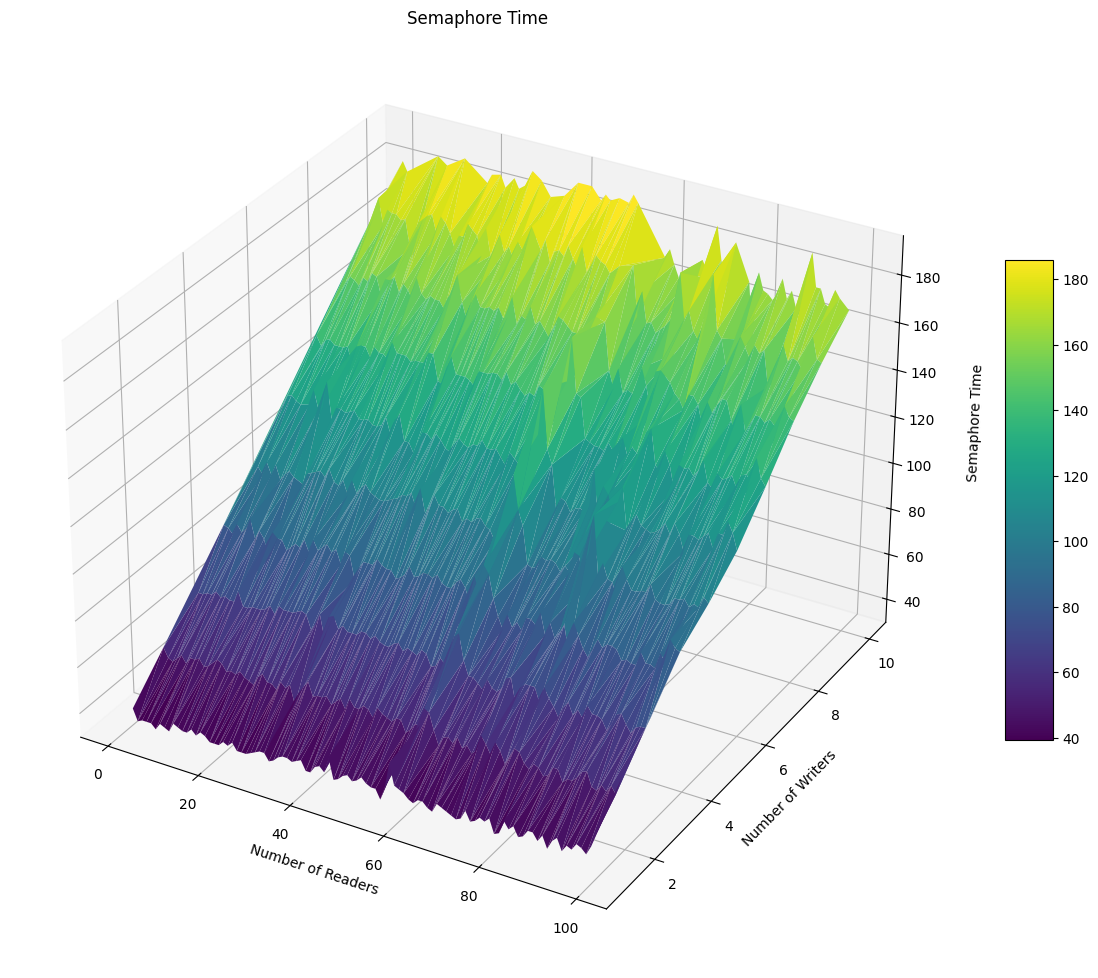
\includegraphics[width=0.6\textwidth]{./semT.png}
\caption{Całkowity czas wykonania dla wersji z semaforami.}
\end{figure}

\begin{figure}[H]
\centering
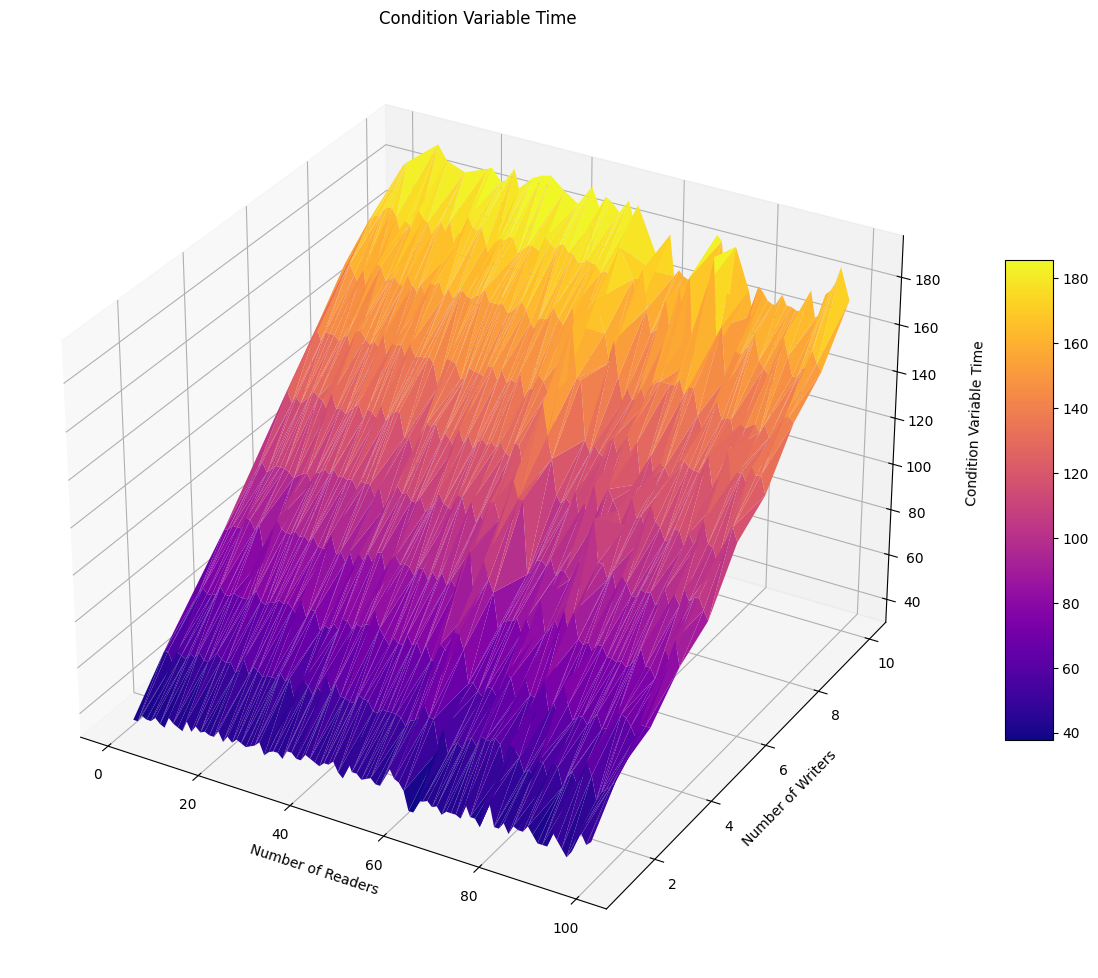
\includegraphics[width=0.6\textwidth]{./condT.png}
\caption{Całkowity czas wykonania dla wersji ze zmiennymi warunkowymi.}
\end{figure}

\begin{figure}[H]
\centering
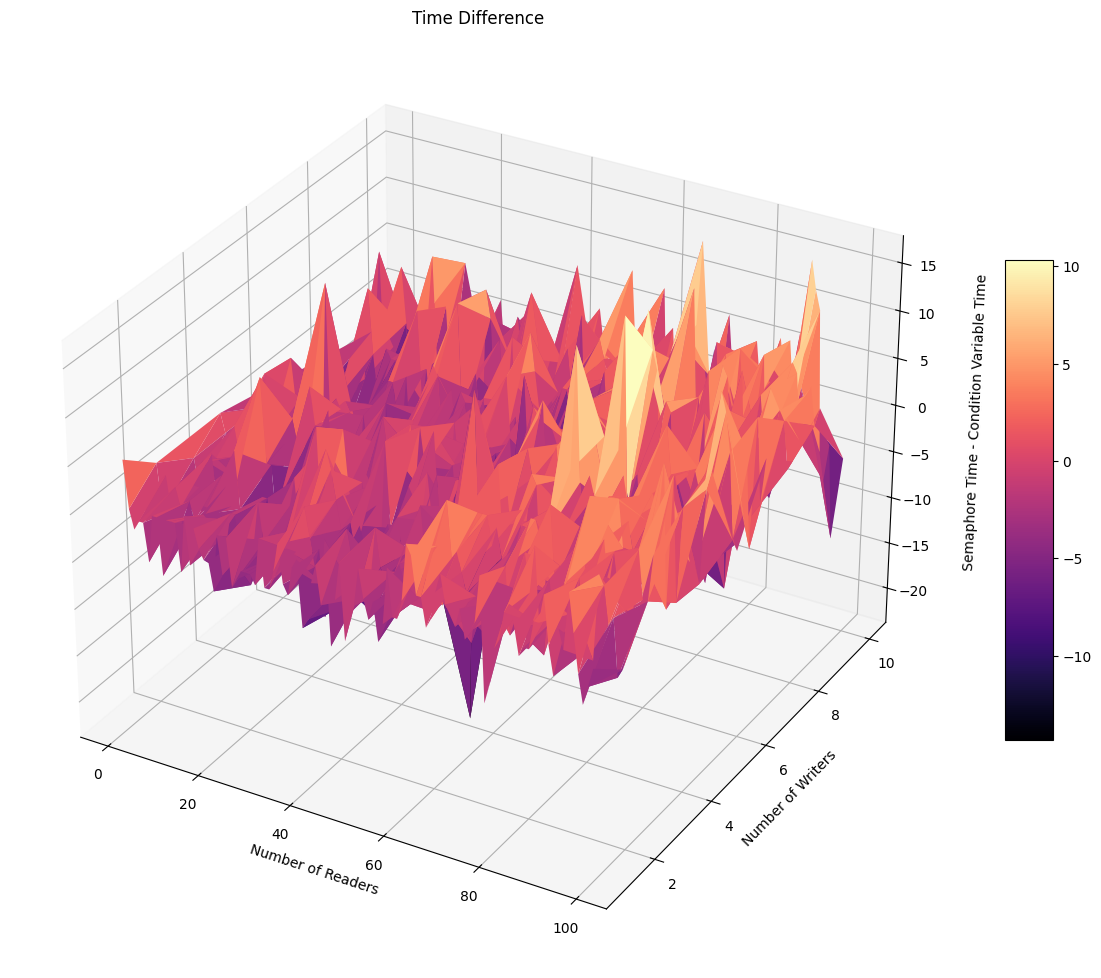
\includegraphics[width=0.6\textwidth]{./semcondT.png}
\caption{Różnica pomiędzy czasem wykoania dla wersji z semaforami i zmiennymi warunkowymi.}
\end{figure}


\textbf{Wnioski}: Całkowity czas wykonania dla obu wersji jest zbliżony, najlepiej
obrazuje to wykres różnicy. Otrzymany kształt wygląda jak zaburzona szumem
płaszczyzna równoległa do płaszczyzny \texttt{xOy}, skupiona na osi \(z\) w otoczeniu zera.
\subsubsection*{Czas wykonania \texttt{read()}}
\label{sec:org8be9021}
\begin{figure}[H]
\centering
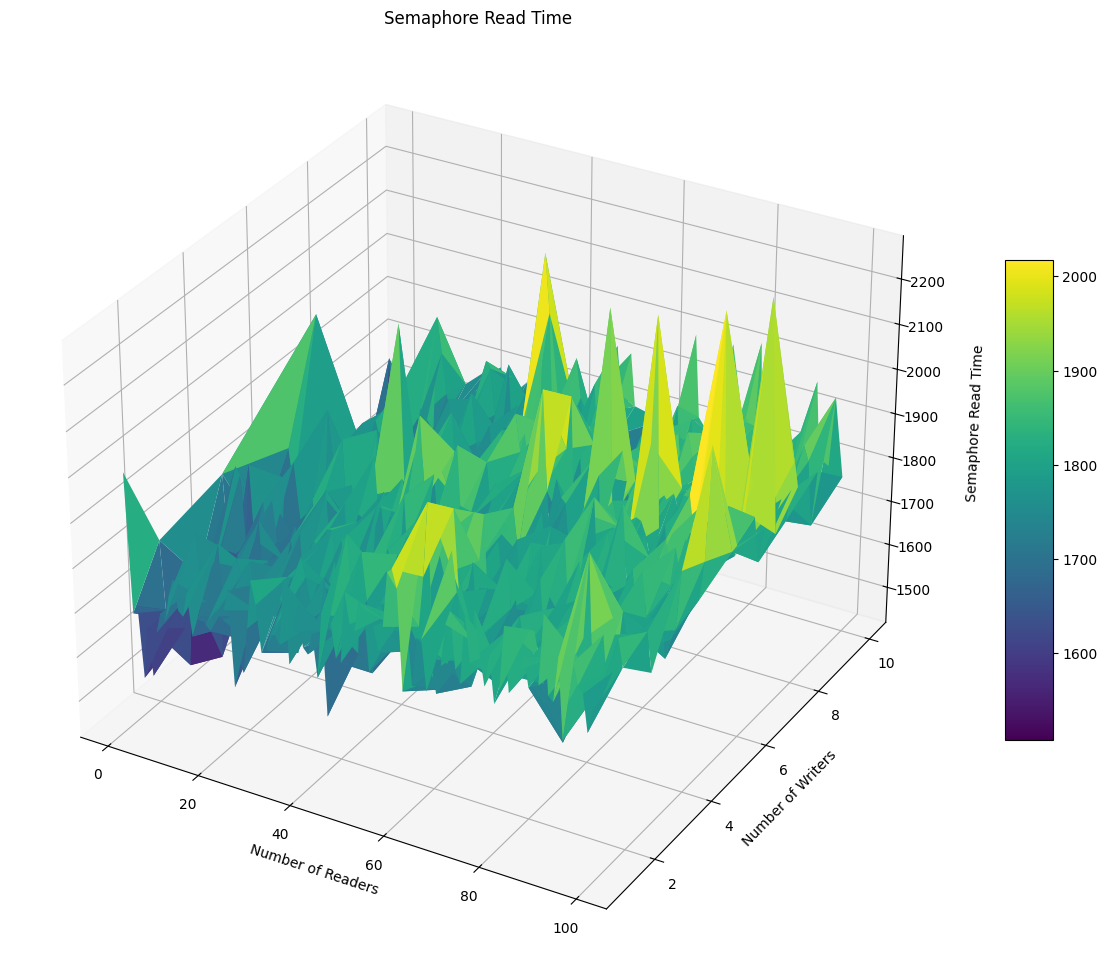
\includegraphics[width=0.6\textwidth]{./semR.png}
\caption{Średni czas wykonania read() dla wersji z semaforami.}
\end{figure}

\begin{figure}[H]
\centering
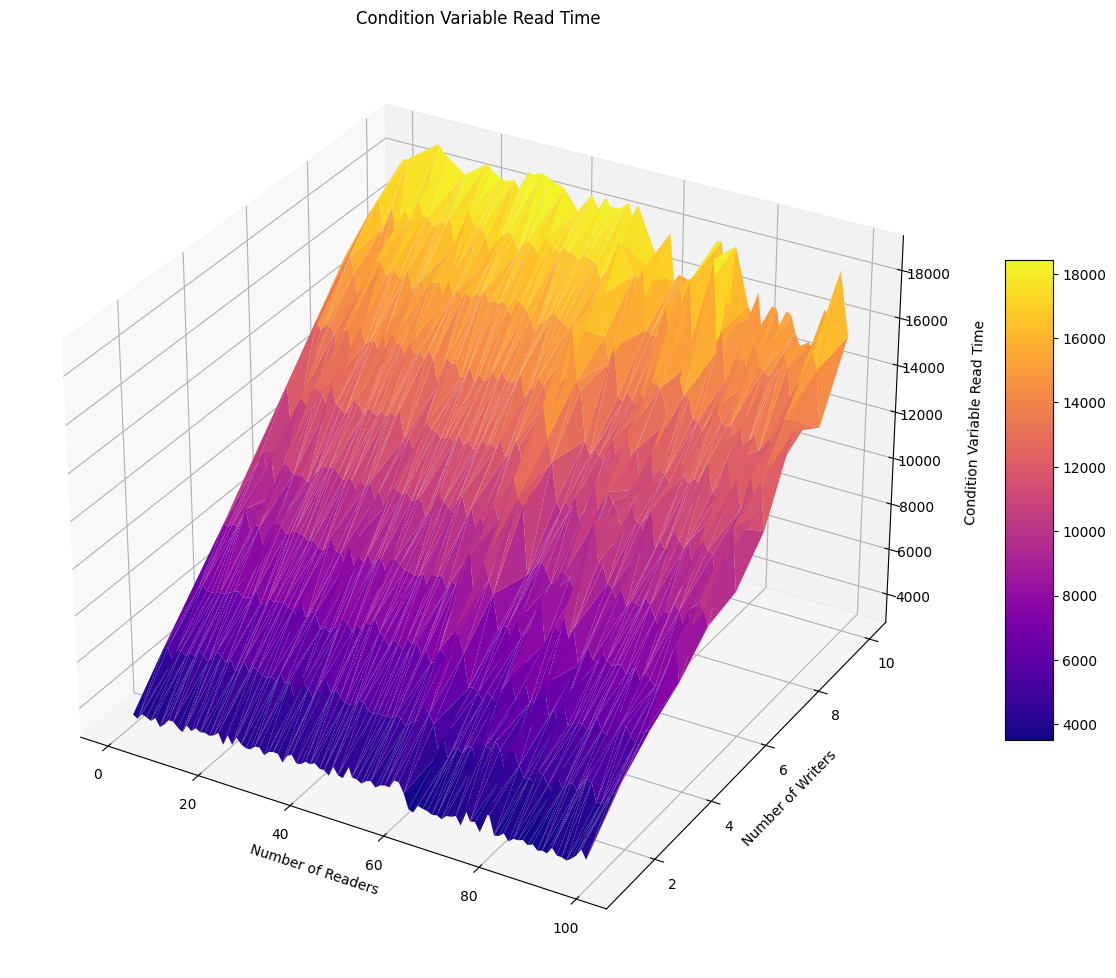
\includegraphics[width=0.6\textwidth]{./condR.png}
\caption{Średni czas wykonania read() dla wersji ze zmiennymi warunkowymi.}
\end{figure}

\begin{figure}[H]
\centering
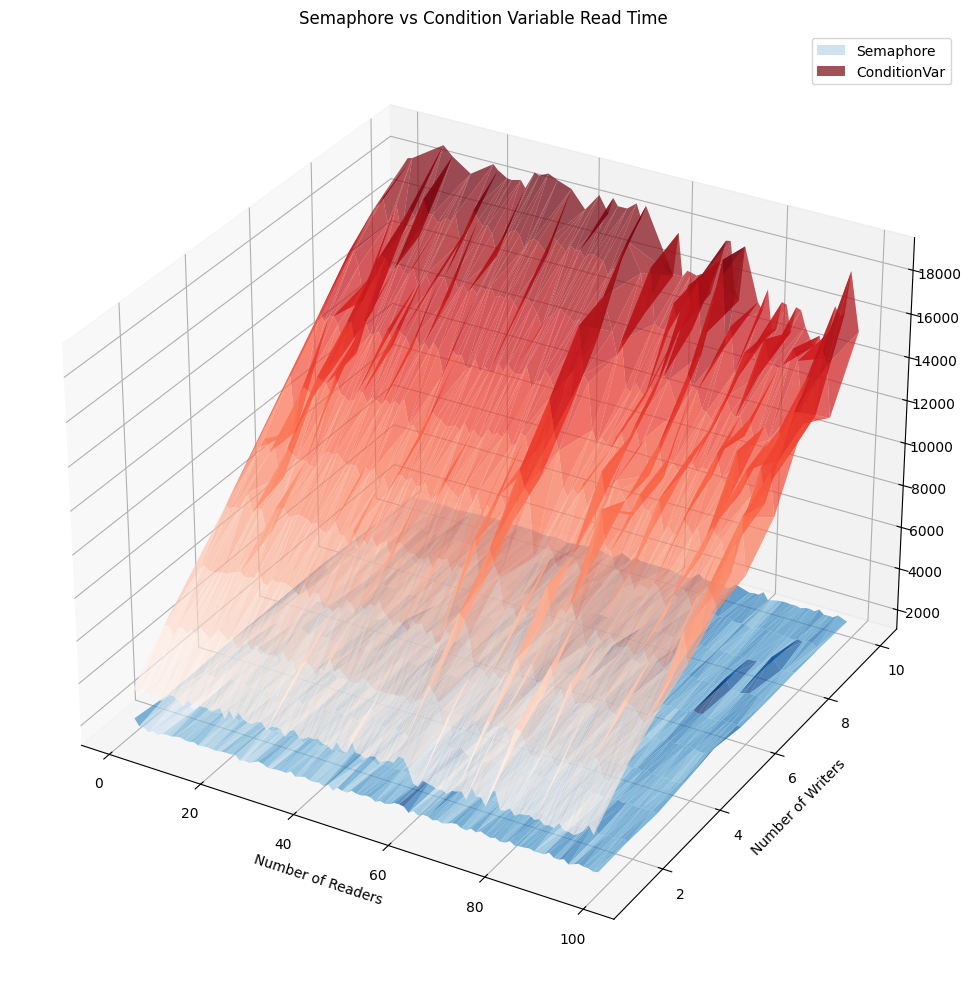
\includegraphics[width=0.6\textwidth]{./semCondR.png}
\caption{Średni czas wykoania read() dla obu wersji.}
\end{figure}


\textbf{Wnioski}: Wersja z semaforami, preferująca czytelników wedle oczekiwań
szybciej wykonuje \texttt{read()}.
 Widzimy, że dla wersji z semaforami, czas
wykonania \texttt{read()} jest w miarę stały, niezależnie od liczby czytelników i pisarzy.
Jest to zrozumiałe, ponieważ czytelnicy mogą wchodzić do biblioteki równolegle,
a obecność oczekujących pisarzy nie wpływa na czas oczekiwania czytelników.
Dla wersji ze zmiennymi warunkowymi, która to preferuje pisarzy, czas wykonania
\texttt{read()} rośnie znacząco z liczbą pisarzy, co jest zrozumiałe, ponieważ czytelnicy
muszą czekać nie tylko na obecnego pisarza, ale również na innych oczekujących.
\subsubsection*{Czas wykonania \texttt{write()}}
\label{sec:org209c3fd}
\begin{figure}[H]
\centering
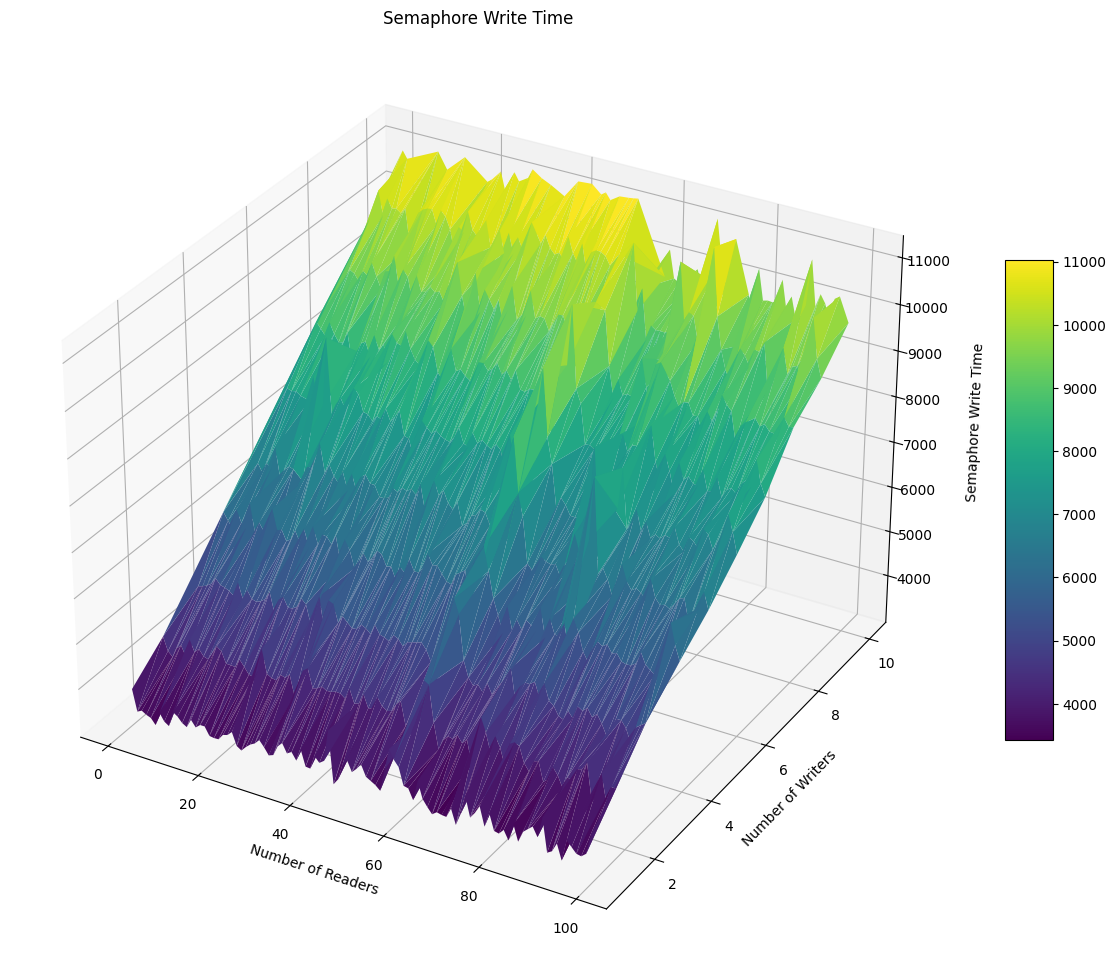
\includegraphics[width=0.6\textwidth]{./semW.png}
\caption{Średni czas wykonania write() dla wersji z semaforami.}
\end{figure}

\begin{figure}[H]
\centering
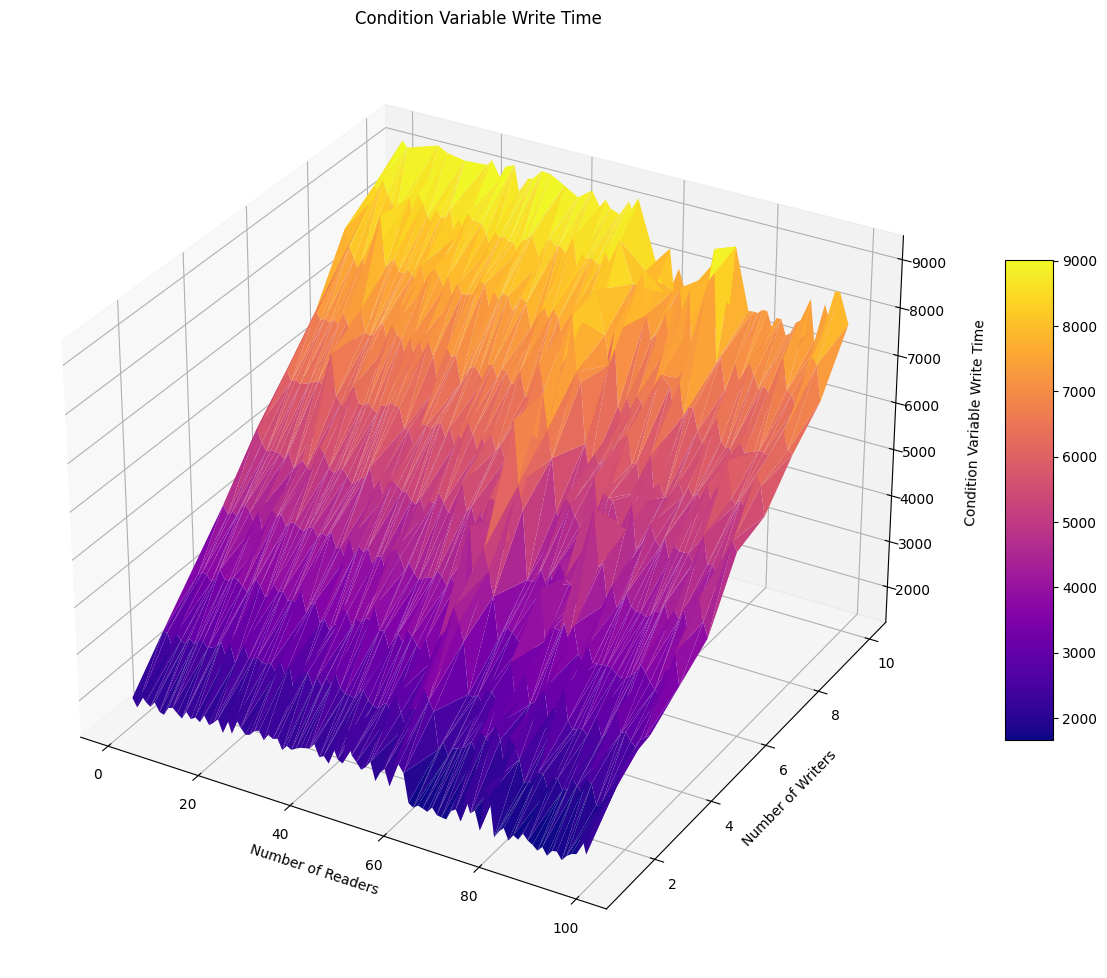
\includegraphics[width=0.6\textwidth]{./condW.png}
\caption{Średni czas wykonania write() dla wersji ze zmiennymi warunkowymi.}
\end{figure}

\begin{figure}[H]
\centering
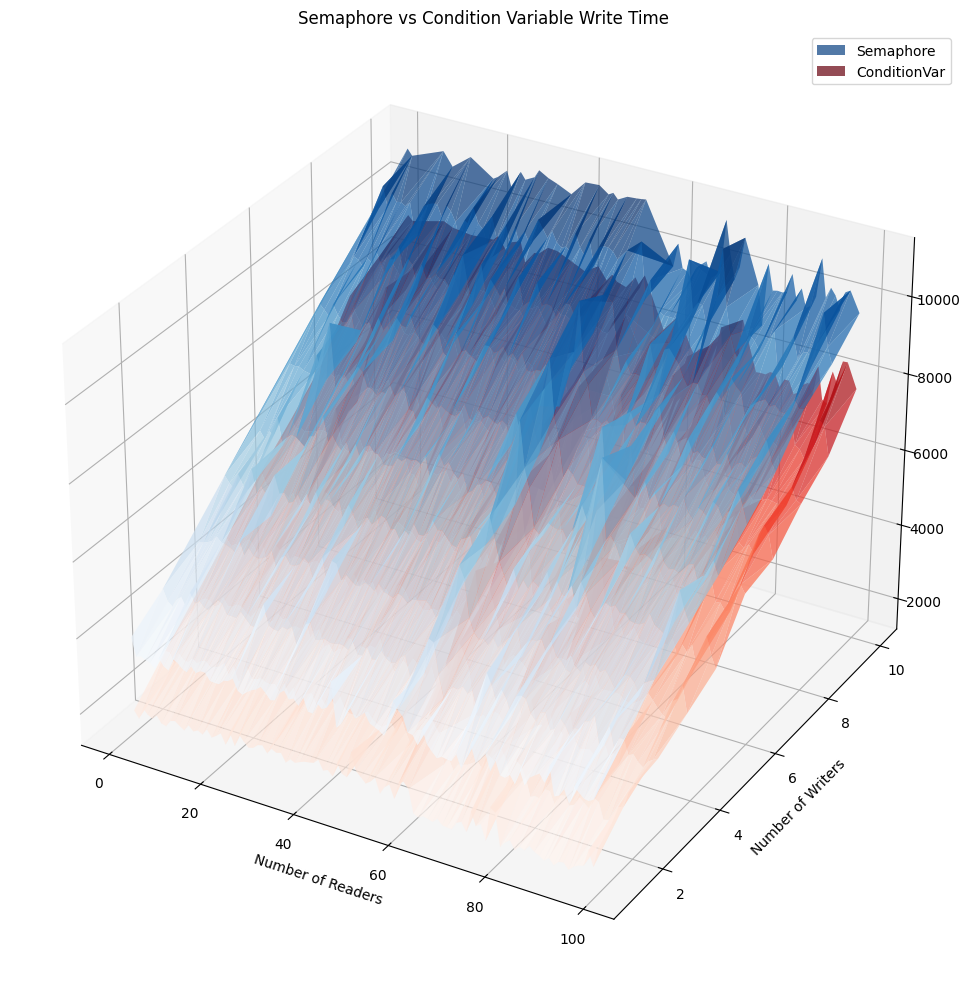
\includegraphics[width=0.6\textwidth]{./semcondW.png}
\caption{Średni czas wykoania write() dla obu wersji.}
\end{figure}


\textbf{Wnioski}: Co ciekawe nie mamy tutaj sytuacji całkowicie symetrycznej z funkcją \texttt{read()}.
Wersja preferująca pisarzy jest wedle oczekiwań szybsza w metodzie \texttt{write()}.
Ale nadal czas ten rośnie wraz z liczbą czytelników, co jest zrozumiałe, ponieważ
pisarze wymagają dostępu wyłącznego do biblioteki.
\subsection*{Podsumowanie}
\label{sec:orgb8c84a6}
Problem czytelników i pisarzy został rozwiązany na dwa sposoby z preferencją dla czytelników
oraz pisarzy. W każdej z zaimplementowanych wersji, istnieje ryzyko
zagłodzenia jednej z grup. Wersję sprawiedliwą można uzyskać np. poprzez zastosowanie
kolejek FIFO. Takie rozwiązanie nosi jednak za sobą duży narzut czasowy.
Zaproponowane dwa rozwiązania różnią się czasem wykonania operacji \texttt{read()} oraz \texttt{write()}.
Jeżeli nasz program o wiele częściej czyta niż pisze, to warto zastosować przedstawioną
wersję z semaforami, bo jest prosta i zapewnia szybkie wykonanie \texttt{read()}.
Jeżeli natomiast zależy nam na jak najszybszym wprowadzaniu zmian w zasobie to możemy zastosować przedstawioną wersję ze zmiennymi warunkowymi.

\newpage
\section*{Zadanie 2}
\label{sec:org5b4f820}
Tworzymy klasę opisującą jeden węzeł listy \texttt{Node}, który zawiera wartość, referencję do następnego węzła oraz zamek.

\begin{Code}
\begin{Verbatim}
\color{EFD}\EFk{class} \EFt{Node} \EFrda{\{}
    \EFt{Object} \EFv{value};
    \EFt{Node} \EFv{next};
    \EFt{Lock} \EFv{lock} = \EFk{new} \EFt{ReentrantLock}\EFrdb{(}\EFrdb{)};

    \EFk{public} Node\EFrdb{(}Object value\EFrdb{)} \EFrdb{\{}
        \EFk{this}\EFrdc{(}value, \EFo{null}\EFrdc{)};
    \EFrdb{\}}

    \EFk{public} Node\EFrdb{(}\EFt{Object} \EFv{value}, Node next\EFrdb{)} \EFrdb{\{}
        \EFk{this}.value = value;
        \EFk{this}.next = next;
    \EFrdb{\}}

    \EFk{public} \EFt{void} \EFf{lock}\EFrdb{(}\EFrdb{)} \EFrdb{\{}
        lock.lock\EFrdc{(}\EFrdc{)};
    \EFrdb{\}}

    \EFk{public} \EFt{void} \EFf{unlock}\EFrdb{(}\EFrdb{)} \EFrdb{\{}
        lock.unlock\EFrdc{(}\EFrdc{)};
    \EFrdb{\}}

    \EFk{public} \EFt{Node} \EFf{getNext}\EFrdb{(}\EFrdb{)} \EFrdb{\{}
        \EFk{return} next;
    \EFrdb{\}}

    \EFk{public} \EFt{void} \EFf{setNext}\EFrdb{(}\EFt{Node} \EFv{next}\EFrdb{)} \EFrdb{\{}
        \EFk{this}.next = next;
    \EFrdb{\}}

    \EFk{public} \EFt{Object} \EFf{getValue}\EFrdb{(}\EFrdb{)} \EFrdb{\{}
        \EFk{return} value;
    \EFrdb{\}}

    \EFk{public} \EFt{void} \EFf{setValue}\EFrdb{(}\EFt{Object} \EFv{value}\EFrdb{)} \EFrdb{\{}
        \EFk{this}.value = value;
    \EFrdb{\}}
\EFrda{\}}
\end{Verbatim}
\end{Code}

Tworzymy interfejs \texttt{MyList}, który zawiera trzy metody podane w zadaniu.
\begin{Code}
\begin{Verbatim}
\color{EFD}\EFk{interface} \EFt{MyList} \EFrda{\{}
    \EFt{boolean} \EFf{remove}\EFrdb{(}\EFt{Object} \EFv{value}\EFrdb{)};
    \EFt{boolean} \EFf{contains}\EFrdb{(}\EFt{Object} \EFv{value}\EFrdb{)};
    \EFt{void} \EFf{add}\EFrdb{(}\EFt{Object} \EFv{value}\EFrdb{)};
\EFrda{\}}
\end{Verbatim}
\end{Code}
\subsection*{Wersja z jednym zamkiem}
\label{sec:org9d274be}
Wykorzystujemy tutaj zamek związany z monitorem obiektu.
Implementacja to standardowe operacje na liście jednokierunkowej.
Przekazujemy czasy operacji porównywania i wstawiania w celu dokonania pomiarów.

\begin{Code}
\begin{Verbatim}
\color{EFD}\EFk{class} \EFt{SingleLockList} \EFk{implements} \EFt{MyList} \EFrda{\{}
    \EFk{private} \EFk{final} \EFt{Node} \EFv{head} = \EFk{new} \EFt{Node}\EFrdb{(}\EFo{null}, \EFo{null}\EFrdb{)};
    \EFk{private} \EFk{final} \EFt{int} \EFv{compareTime};
    \EFk{private} \EFk{final} \EFt{int} \EFv{insertTime};

    \EFk{public} SingleLockList\EFrdb{(}\EFt{int} \EFv{compareTime}, \EFt{int} \EFv{insertTime}\EFrdb{)} \EFrdb{\{}
        \EFk{this}.compareTime = compareTime;
        \EFk{this}.insertTime= insertTime;
    \EFrdb{\}}

    \textcolor[HTML]{0000b0}{@Override}
    \EFk{public} \EFk{synchronized} \EFt{boolean} \EFf{remove}\EFrdb{(}\EFt{Object} \EFv{value}\EFrdb{)} \EFrdb{\{}
        \EFt{Node} \EFv{pred} = head;
        \EFt{Node} \EFv{curr} = head.getNext\EFrdc{(}\EFrdc{)};
        \EFk{while} \EFrdc{(}curr != \EFo{null}\EFrdc{)} \EFrdc{\{}
            \EFk{try} \EFrdd{\{}
                Thread.sleep\EFrda{(}compareTime\EFrda{)};
            \EFrdd{\}} \EFk{catch} \EFrdd{(}Exception ignored\EFrdd{)} \EFrdd{\{}
            \EFrdd{\}}

            \EFk{if} \EFrdd{(}curr.getValue\EFrda{(}\EFrda{)}.equals\EFrda{(}value\EFrda{)}\EFrdd{)} \EFrdd{\{}
                pred.setNext\EFrda{(}curr.getNext\EFrdb{(}\EFrdb{)}\EFrda{)};
                \EFk{return} \EFo{true};
            \EFrdd{\}}

            pred = curr;
            curr = curr.getNext\EFrdd{(}\EFrdd{)};
        \EFrdc{\}}
        \EFk{return} \EFo{false};
    \EFrdb{\}}

    \textcolor[HTML]{0000b0}{@Override}
    \EFk{public} \EFk{synchronized} \EFt{boolean} \EFf{contains}\EFrdb{(}\EFt{Object} \EFv{value}\EFrdb{)} \EFrdb{\{}
        \EFt{Node} \EFv{curr} = head.getNext\EFrdc{(}\EFrdc{)};
        \EFk{while} \EFrdc{(}curr != \EFo{null}\EFrdc{)} \EFrdc{\{}
            \EFk{try} \EFrdd{\{}
                Thread.sleep\EFrda{(}compareTime\EFrda{)};
            \EFrdd{\}} \EFk{catch} \EFrdd{(}Exception ignored\EFrdd{)} \EFrdd{\{}
            \EFrdd{\}}

            \EFk{if} \EFrdd{(}curr.getValue\EFrda{(}\EFrda{)}.equals\EFrda{(}value\EFrda{)}\EFrdd{)} \EFrdd{\{}
                \EFk{return} \EFo{true};
            \EFrdd{\}}

            curr = curr.getNext\EFrdd{(}\EFrdd{)};
        \EFrdc{\}}
        \EFk{return} \EFo{false};
    \EFrdb{\}}

    \textcolor[HTML]{0000b0}{@Override}
    \EFk{public} \EFk{synchronized} \EFt{void} \EFf{add}\EFrdb{(}\EFt{Object} \EFv{value}\EFrdb{)} \EFrdb{\{}
        \EFt{Node} \EFv{last} = head;
        \EFk{while} \EFrdc{(}last.getNext\EFrdd{(}\EFrdd{)} != \EFo{null}\EFrdc{)} \EFrdc{\{}
            last = last.getNext\EFrdd{(}\EFrdd{)};
        \EFrdc{\}}

        \EFk{try} \EFrdc{\{}
            Thread.sleep\EFrdd{(}insertTime\EFrdd{)};
        \EFrdc{\}} \EFk{catch} \EFrdc{(}Exception ignored\EFrdc{)} \EFrdc{\{}
        \EFrdc{\}}

        last.setNext\EFrdc{(}\EFk{new} \EFt{Node}\EFrdd{(}value\EFrdd{)}\EFrdc{)};
    \EFrdb{\}}
\EFrda{\}}
\end{Verbatim}
\end{Code}
\subsection*{Wersja z zamkiem na jeden element}
\label{sec:org8483b7e}
Implementacja wszystkich metod w tej wersji, opiera się
na prostym schemacie działania:
\begin{enumerate}
\item zamknij zamek na pierwszym elemencie listy
\item zamknij zamek na drugim elemencie
\item otwórz zamek na pierwszym elemencie
\item zamknij zamek na trzecim elemencie
\item otwórz zamek na drugim elemencie
\item powtarzaj dla kolejnych elementów
\end{enumerate}

Dzięki temu nie musimy blokować całej listy, co
oznacza że jeżeli np. dany wątek wykonuje operację \texttt{add()}
i przeszedł już kilka pierwszych elementów to drugi
wątek może zacząć przeglądać ten początek w celu np.
sprawdzenia czy istnieje dany element w liście.

\begin{Code}
\begin{Verbatim}
\color{EFD}\EFk{class} \EFt{LockPerElementList} \EFk{implements} \EFt{MyList} \EFrda{\{}
    \EFk{private} \EFk{final} \EFt{Node} \EFv{head} = \EFk{new} \EFt{Node}\EFrdb{(}\EFo{null}, \EFo{null}\EFrdb{)};
    \EFk{private} \EFk{final} \EFt{int} \EFv{compareTime};
    \EFk{private} \EFk{final} \EFt{int} \EFv{insertTime};

    \EFk{public} LockPerElementList\EFrdb{(}\EFt{int} \EFv{compareTime}, \EFt{int} \EFv{insertTime}\EFrdb{)} \EFrdb{\{}
        \EFk{this}.compareTime = compareTime;
        \EFk{this}.insertTime = insertTime;
    \EFrdb{\}}

    \textcolor[HTML]{0000b0}{@Override}
    \EFk{public} \EFt{boolean} \EFf{remove}\EFrdb{(}\EFt{Object} \EFv{value}\EFrdb{)} \EFrdb{\{}
        \EFt{Node} \EFv{prev} = head;
        \EFt{Node} \EFv{curr} = \EFo{null};
        \EFk{try} \EFrdc{\{}
            prev.lock\EFrdd{(}\EFrdd{)};
            curr = prev.getNext\EFrdd{(}\EFrdd{)};
            \EFk{while} \EFrdd{(}curr != \EFo{null}\EFrdd{)} \EFrdd{\{}
                curr.lock\EFrda{(}\EFrda{)};
                \EFk{try} \EFrda{\{}
                    Thread.sleep\EFrdb{(}compareTime\EFrdb{)};
                \EFrda{\}} \EFk{catch} \EFrda{(}Exception ignored\EFrda{)} \EFrda{\{}
                \EFrda{\}}

                \EFk{if} \EFrda{(}curr.getValue\EFrdb{(}\EFrdb{)}.equals\EFrdb{(}value\EFrdb{)}\EFrda{)} \EFrda{\{}
                    prev.setNext\EFrdb{(}curr.getNext\EFrdc{(}\EFrdc{)}\EFrdb{)};
                    \EFk{return} \EFo{true};
                \EFrda{\}}

                prev.unlock\EFrda{(}\EFrda{)};
                prev = curr;
                curr = prev.getNext\EFrda{(}\EFrda{)};
            \EFrdd{\}}
        \EFrdc{\}} \EFk{finally} \EFrdc{\{}
            \EFk{if} \EFrdd{(}curr != \EFo{null}\EFrdd{)} \EFrdd{\{}
                curr.unlock\EFrda{(}\EFrda{)};
            \EFrdd{\}}
            prev.unlock\EFrdd{(}\EFrdd{)};
        \EFrdc{\}}

        \EFk{return} \EFo{false};
    \EFrdb{\}}

    \textcolor[HTML]{0000b0}{@Override}
    \EFk{public} \EFt{boolean} \EFf{contains}\EFrdb{(}\EFt{Object} \EFv{value}\EFrdb{)} \EFrdb{\{}
        \EFt{Node} \EFv{prev} = head;
        \EFt{Node} \EFv{curr} = \EFo{null};

        \EFk{try} \EFrdc{\{}
            prev.lock\EFrdd{(}\EFrdd{)};
            curr = prev.getNext\EFrdd{(}\EFrdd{)};
            \EFk{while} \EFrdd{(}curr != \EFo{null}\EFrdd{)} \EFrdd{\{}
                curr.lock\EFrda{(}\EFrda{)};
                \EFk{try} \EFrda{\{}
                    Thread.sleep\EFrdb{(}compareTime\EFrdb{)};
                \EFrda{\}} \EFk{catch} \EFrda{(}Exception ignored\EFrda{)} \EFrda{\{}
                \EFrda{\}}

                \EFk{if} \EFrda{(}curr.getValue\EFrdb{(}\EFrdb{)}.equals\EFrdb{(}value\EFrdb{)}\EFrda{)} \EFrda{\{}
                    \EFk{return} \EFo{true};
                \EFrda{\}}

                prev.unlock\EFrda{(}\EFrda{)};
                prev = curr;
                curr = prev.getNext\EFrda{(}\EFrda{)};
            \EFrdd{\}}
        \EFrdc{\}} \EFk{finally} \EFrdc{\{}
            \EFk{if} \EFrdd{(}curr != \EFo{null}\EFrdd{)} \EFrdd{\{}
                curr.unlock\EFrda{(}\EFrda{)};
            \EFrdd{\}}
            prev.unlock\EFrdd{(}\EFrdd{)};
        \EFrdc{\}}
        \EFk{return} \EFo{false};
    \EFrdb{\}}

    \textcolor[HTML]{0000b0}{@Override}
    \EFk{public} \EFt{void} \EFf{add}\EFrdb{(}\EFt{Object} \EFv{value}\EFrdb{)} \EFrdb{\{}
        \EFt{Node} \EFv{curr} = head;

        \EFk{try} \EFrdc{\{}
            curr.lock\EFrdd{(}\EFrdd{)};
            \EFt{Node} \EFv{next} = curr.getNext\EFrdd{(}\EFrdd{)};


            \EFk{while} \EFrdd{(}next != \EFo{null}\EFrdd{)} \EFrdd{\{}
                next.lock\EFrda{(}\EFrda{)};

                curr.unlock\EFrda{(}\EFrda{)};
                curr = next;
                next = curr.getNext\EFrda{(}\EFrda{)};
            \EFrdd{\}}

            \EFk{try} \EFrdd{\{}
                Thread.sleep\EFrda{(}insertTime\EFrda{)};
            \EFrdd{\}} \EFk{catch} \EFrdd{(}Exception ignored\EFrdd{)} \EFrdd{\{}
            \EFrdd{\}}

            curr.setNext\EFrdd{(}\EFk{new} \EFt{Node}\EFrda{(}value\EFrda{)}\EFrdd{)};
        \EFrdc{\}} \EFk{finally} \EFrdc{\{}
            curr.unlock\EFrdd{(}\EFrdd{)};
        \EFrdc{\}}
    \EFrdb{\}}
\EFrda{\}}
\end{Verbatim}
\end{Code}
\subsection*{Kod testujący}
\label{sec:org361352c}
Tworzymy 4 wątki \texttt{Worker}, które wykonują operacje \texttt{add}, \texttt{remove}, \texttt{contains} na liście.
Operacje dla nich są losowe. Mierzymy jedynie czas wykonania. Wynikiem
programu jest tabela w formacie \texttt{.csv}.

\begin{Code}
\begin{Verbatim}
\color{EFD}\EFk{class} \EFt{Worker} \EFk{implements} \EFt{Runnable} \EFrda{\{}
    \EFk{private} \EFk{final} \EFt{MyList} \EFv{list};
    \EFk{private} \EFk{final} \EFt{List}\EFrdb{<}\EFt{Character}\EFrdb{>} \EFv{operations};

    \EFk{public} Worker\EFrdb{(}\EFt{MyList} \EFv{list}, \EFt{List}\EFrdc{<}\EFt{Character}\EFrdc{>} \EFv{operations}\EFrdb{)} \EFrdb{\{}
        \EFk{this}.list = list;
        \EFk{this}.operations = operations;
    \EFrdb{\}}

    \textcolor[HTML]{0000b0}{@Override}
    \EFk{public} \EFt{void} \EFf{run}\EFrdb{(}\EFrdb{)} \EFrdb{\{}
        \EFk{for} \EFrdc{(}\EFt{Character} \EFv{operation} : operations\EFrdc{)} \EFrdc{\{}
            \EFk{switch} \EFrdd{(}operation\EFrdd{)} \EFrdd{\{}
                \EFk{case} \EFs{'a'} -> list.add\EFrda{(}ThreadLocalRandom.current\EFrdb{(}\EFrdb{)}.nextInt\EFrdb{(}\EFhn{30}\EFrdb{)}\EFrda{)};
                \EFk{case} \EFs{'r'} -> list.remove\EFrda{(}ThreadLocalRandom.current\EFrdb{(}\EFrdb{)}.nextInt\EFrdb{(}\EFhn{30}\EFrdb{)}\EFrda{)};
                \EFk{case} \EFs{'c'} -> list.contains\EFrda{(}ThreadLocalRandom.current\EFrdb{(}\EFrdb{)}.nextInt\EFrdb{(}\EFhn{30}\EFrdb{)}\EFrda{)};
            \EFrdd{\}}
        \EFrdc{\}}

    \EFrdb{\}}
\EFrda{\}}

\EFk{public} \EFk{class} \EFt{ConcurrentLinkedList} \EFrda{\{}
    \EFk{public} \EFk{static} \EFt{void} \EFf{main}\EFrdb{(}\EFt{String}\EFrdc{[}\EFrdc{]} \EFv{args}\EFrdb{)} \EFrdb{\{}
        System.out.println\EFrdc{(}\EFs{"insertTime,compareTime,SingleLockList,LockPerElementList"}\EFrdc{)};

        \EFk{for} \EFrdc{(}\EFt{int} \EFv{insertTime} = \EFhn{1}; insertTime <= \EFhn{10}; insertTime++\EFrdc{)} \EFrdc{\{}
            \EFk{for} \EFrdd{(}\EFt{int} \EFv{compareTime} = \EFhn{1}; compareTime <= \EFhn{10}; compareTime++\EFrdd{)} \EFrdd{\{}
                \EFt{var} \EFv{singleLockList} = \EFk{new} \EFt{SingleLockList}\EFrda{(}compareTime, insertTime\EFrda{)};
                \EFt{var} \EFv{lockPerElementList} = \EFk{new} \EFt{LockPerElementList}\EFrda{(}compareTime, insertTime\EFrda{)};
                \EFt{long} \EFv{singleLockListTime} = avgTestCase\EFrda{(}singleLockList\EFrda{)};

                \EFt{long} \EFv{lockPerElementListTime} = avgTestCase\EFrda{(}lockPerElementList\EFrda{)};

                System.out.println\EFrda{(}insertTime + \EFs{","} +
                                   compareTime + \EFs{","} +
                                   singleLockListTime + \EFs{","} +
                                   lockPerElementListTime\EFrda{)};
            \EFrdd{\}}
        \EFrdc{\}}


    \EFrdb{\}}


    \EFk{private} \EFk{static} \EFt{long} \EFf{avgTestCase}\EFrdb{(}\EFt{MyList} \EFv{list}\EFrdb{)} \EFrdb{\{}
        \EFk{final} \EFt{int} \EFv{amountOfTests} = \EFhn{3};
        \EFt{long} \EFv{sum} = \EFhn{0};
        \EFk{for} \EFrdc{(}\EFt{int} \EFv{i} = \EFhn{0}; i < \EFt{amountOfTests}; i++\EFrdc{)} \EFrdc{\{}
            sum += testCase\EFrdd{(}list\EFrdd{)};
        \EFrdc{\}}
        \EFk{return} sum / amountOfTests;
    \EFrdb{\}}

    \EFk{private} \EFk{static} \EFt{long} \EFf{testCase}\EFrdb{(}\EFt{MyList} \EFv{list}\EFrdb{)} \EFrdb{\{}
        \EFt{var} \EFv{threads} = \EFk{new} \EFt{ArrayList}\EFrdc{<}\EFt{Thread}\EFrdc{>}\EFrdc{(}\EFrdc{)};
        \EFk{final} \EFt{int} \EFv{amountOfThreads} = \EFhn{4};
        \EFk{final} \EFt{int} \EFv{amountOfOperations} = \EFhn{25};
        \EFt{Random} \EFv{random} = \EFk{new} \EFt{Random}\EFrdc{(}\EFrdc{)};


        \EFk{for} \EFrdc{(}\EFt{int} \EFv{i} = \EFhn{0}; i < \EFt{amountOfThreads}; i++\EFrdc{)} \EFrdc{\{}
            \EFt{var} \EFv{operations} = \EFk{new} \EFt{ArrayList}\EFrdd{<}\EFt{Character}\EFrdd{>}\EFrdd{(}\EFrdd{)};
            \EFk{for} \EFrdd{(}\EFt{int} \EFv{j} = \EFhn{0}; j < \EFt{amountOfOperations}; j++\EFrdd{)} \EFrdd{\{}
                \EFk{final} \EFt{int} \EFv{operation} = random.nextInt\EFrda{(}\EFhn{3}\EFrda{)};
                \EFk{switch} \EFrda{(}operation\EFrda{)} \EFrda{\{}
                    \EFk{case} \EFhn{0} -> operations.add\EFrdb{(}\EFs{'a'}\EFrdb{)};
                    \EFk{case} \EFhn{1} -> operations.add\EFrdb{(}\EFs{'r'}\EFrdb{)};
                    \EFk{case} \EFhn{2} -> operations.add\EFrdb{(}\EFs{'c'}\EFrdb{)};
                \EFrda{\}}
            \EFrdd{\}}
            threads.add\EFrdd{(}\EFk{new} \EFt{Thread}\EFrda{(}\EFk{new} \EFt{Worker}\EFrdb{(}list, operations\EFrdb{)}\EFrda{)}\EFrdd{)};
        \EFrdc{\}}

        \EFt{var} \EFv{startTime} = System.currentTimeMillis\EFrdc{(}\EFrdc{)};
        threads.forEach\EFrdc{(}Thread::start\EFrdc{)};
        threads.forEach\EFrdc{(}t -> \EFrdd{\{}
            \EFk{try} \EFrda{\{}
                t.join\EFrdb{(}\EFrdb{)};
            \EFrda{\}} \EFk{catch} \EFrda{(}InterruptedException e\EFrda{)} \EFrda{\{}
                e.printStackTrace\EFrdb{(}\EFrdb{)};
            \EFrda{\}}
        \EFrdd{\}}\EFrdc{)};
        \EFt{var} \EFv{endTime} = System.currentTimeMillis\EFrdc{(}\EFrdc{)};
        \EFk{return} endTime - startTime;
    \EFrdb{\}}
\EFrda{\}}
\end{Verbatim}
\end{Code}
\subsection*{Wykresy}
\label{sec:org8be14fd}
Wykorzystując wyjście programu testującego tworzymy wykresy 3D, które przedstawiają czas wykonania
w zależności od czasu operacji porównywania i wstawiania.
Czasy na osiach \texttt{x} oraz \texttt{y} są w milisekundach.

\begin{figure}[H]
\centering
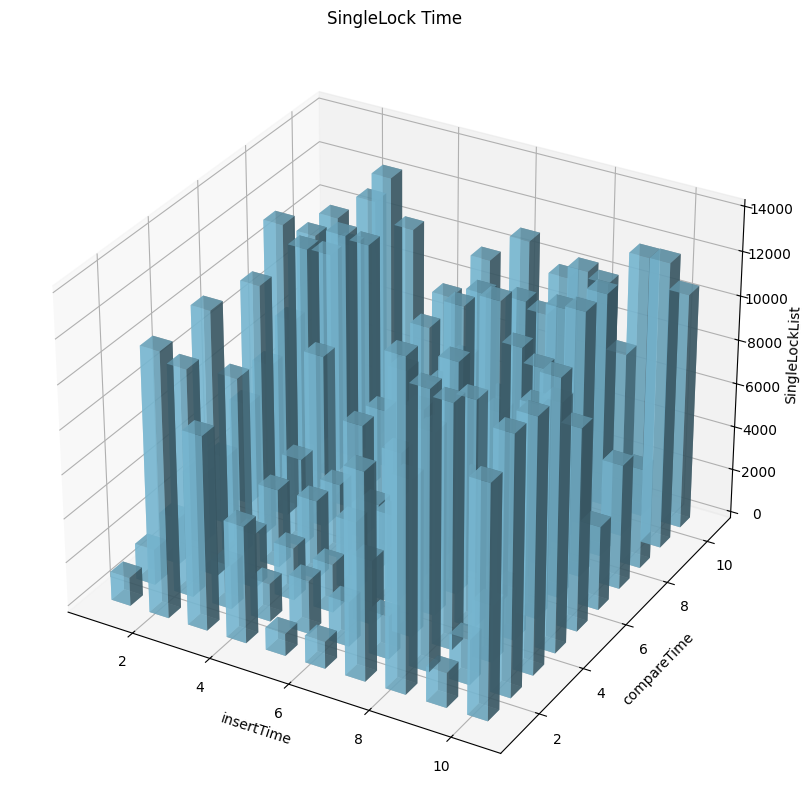
\includegraphics[width=0.5\textwidth]{./sing.png}
\caption{Całkowity czas wykonania dla wersji z jednym zamkiem.}
\end{figure}

\begin{figure}[H]
\centering
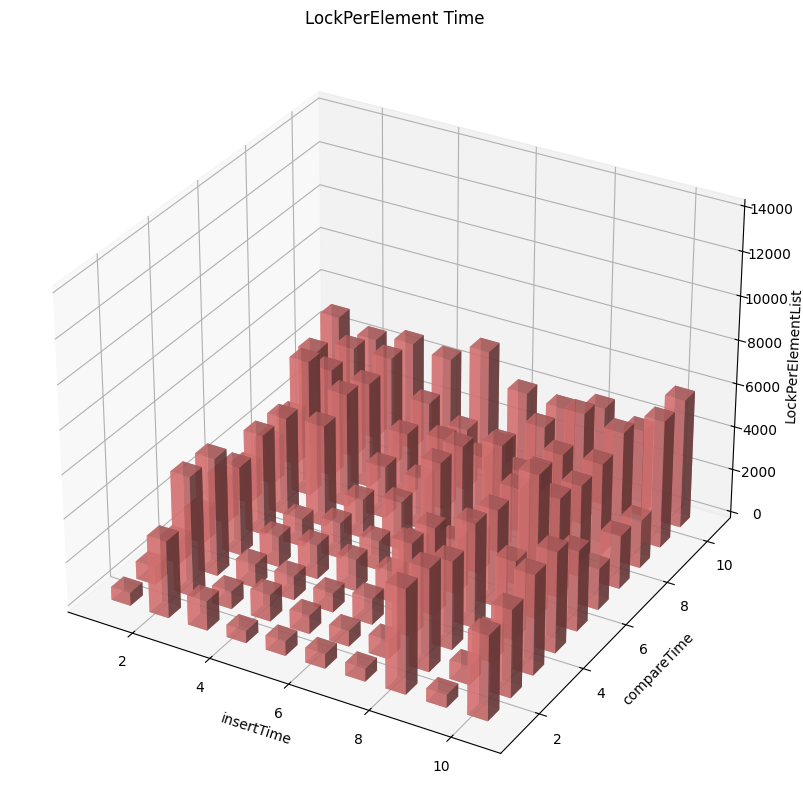
\includegraphics[width=0.5\textwidth]{./pe.png}
\caption{Całkowity czas wykonania dla wersji z zamkiem na jeden element.}
\end{figure}

\textbf{Wnioski}: Wedle oczekiwań wersja z drobnoziarnistym blokowaniem jest szybsza,
bo pozwala na wykonywania wielu operacji równolegle.
Choć jej implementacja jest bardziej skomplikowana, to jednak
przyśpieszenie jest znaczące.
Ten przykład pokazuje, że czasami tworzenie struktur
współbieżnych to nie zawsze jedynie założenie blokady na całą strukturę.
\section*{Bibliografia}
\label{sec:org7eef782}
\begin{itemize}
\item \href{https://en.wikipedia.org/wiki/Readers\%E2\%80\%93writers\_problem}{Problem  czytelników i pisarzy}
\end{itemize}
\end{document}
